%!/usr/bin/env pdflatex
%-*- coding: utf-8 -*-
%@author : Romain Graux
%@date : 2022 June 05, 10:34:48
%@last modified : 2022 June 16, 00:24:41


In this section, we want to build a complete pipeline from a raw point cloud to a DNA strand that will be later synthestized in a medium and kept for a long period (Could be dozen or even hundred of years). After this long period of time, we would like to recover our point cloud as faithful as possible to the original. 

We thus have all the building blocks to construct this pipeline and be able to encode and decode point clouds. However, this pipeline will not be constructed to be the most efficient and optimized DNA code point cloud compression algorithm but it will be a baseline on which we can base ourselves to compare future models. 

% TIKZ pour representer le full pipeline


\section{Point cloud latent representation}

The first step is to turn the point cloud into a smaller latent representation. For this purpose, we can use the point cloud compression model previously described in section \ref{sec:pcc} that has already learned the principal features of point clouds. 

The latent representation $y$ contains a compressed representation with less information but still all the necessary information to reconstruct the original point cloud. From a block of shape $k \times k \times k$, once passed through the Analysis Transform, the latent reprsentation $y$ has a shape $\lceil\frac{k}{8}\rceil \times \lceil\frac{k}{8}\rceil \times \lceil\frac{k}{8}\rceil \times d$ with $d$ being the arbitrary latent depth. Therefore if the latent depth $d$ is well chosen, the latent representation contains all information to retrieve the original point cloud while being smaller.

In our particular implementation, we chose a latent depth of $160$ which means that we indeed have a smaller shape since $8 \times 8 \times 8 \geq 160$. 

We also have to make a choice on which model to use for the transfer learning of the weights since several models are available for different bitrate/distortion tradeoffs. As we will see in the next sections, the nucleotiderate mostly depends on the input shape without impacting the distortion no matter which one is chosen. Thus to get the best reconstruction possible, we will choose the highest $\lambda$ value (1750) for the model. The $\lambda$ value is weighting the focal loss in the global loss used to train the model as explained in Section~\ref{sec:pcc}.

Now that we have a latent representation, we have to go to the next step, which is the JPEG DNA codec described in section \ref{subsec:jpegdna}, but this codec has some requierements that have to be met in order to achieve the best quality, nucleotide rate, all these details will be discuss in the next section.

\section{Latent representation with JPEG DNA codec}

In this part, we will use the JPEG DNA codec but not the full one, we will drop all the part related to JPEG and thus encode directly the coefficients that are normally produced by the last DCT transform. So the input of the codec will be quantized discrete coefficients. To meet these requirements, we will have to change few things from the latent representation $y$.

\subsection{Dimensionality}

The output of the Analysis block is a $l \times l \times l \times d$ latent representation $y$ but since the codec is built for image purpose, it only accepts an image as input which is either of shape $H \times W$ (gray image) or $H \times W \times 3$ (RGB image). 
Consequently, we have to tweak our latent representation $y$ so that it satisfies this requirement, we have several possibilities for that, I tried two different approaches:

\begin{itemize}
    \item The first approach is to merge the two inner dimension together, in that case we have a $l \times l^2 \times d$ shape. We can then encode several $l \times l^2$ images alogn the latent features dimension. This approach allows to process each feature "independently";
    \item The second approach is more simple and consists of merging the three first dimensions together, hence we end up with a $l^3 \times d$ image. We can thus encode directly the full image with the codec.
\end{itemize}

Each approach has its own pros and cons. 

The first one aims at treating each feature separately so that we can encode regarding each feature distribution and hope for less quantized values and in the end, a smaller number of oligos. Although, when encoding the final flat nucleotide stream, we have to add the length of each latent oligo length which is avoidable.

The second as for it, is easier to compute since it is a single gray image like, so we have in the end directly a flat nucleotide stream for a block. 

Finally, as the first one does not offer better performance while enlarging the final stream length (and thus impact the final nucleotiderate), we will simply merge the first three dimensions (dimensions of the feature block) as proposed in the second approach to produce a $2$D tensor compatible with the codec.

\subsection{Quantization}
\label{subsec:quantization}

The other important aspect of the codec is the value type. The Analysis block produces continuous values $y \in [-\inf, \inf]$ due to the nature of convolutional layer and the linear activation function of the last layer but the codec is built to encode discrete integer values as it is the case for the DCT coefficients. This means that we have to convert the latent representation $y$ to an integer value type while ensuring the $y$ range is mapped to a range $[0, span]$ as a bijective maneer. Here the $span$ value is fixed value chosen at compression time as a quality parameter. It is used as a nucleotiderate/distortion tradeoff. The greater the $span$ value, the better the quality and the greater the nucleotiderate. 
Contrastly, the lower the $span$ value, the worse the quality and the lower the nucleotiderate.

To implement such a quantization transform, we can naively do a linear mapping between $[\min{y}, \max{y}]$ to $[0, span]$. With this transform, we create $span+1$ ranges of equal length $\dfrac{\max{y} - \min{y}}{span}$ in which the $y$ values will fall. 
It assumes that $y$ is uniformly distributed because it gives the same range length in which to fall for each $y$ value.

Finally, to get the quantized integer value, we can simply round the final mapped values and it will gives us at most $span+1$ integer values to encode with the JPEG DNA codec.

The mapping can simply be described as: 
$$z = \text{round} \left(span \frac{y - \min{y}}{\max{y} - \min{y}}\right)$$.

\subsection{DCT}

In the original JPEG codec, each $8 \times 8$ block of the images are first centered around $0$ (simply shift by $-128$) and then transformed into the $8 \times 8$ DCT values before being quantized with a default perceptual quantization table. 
For our purposes, we will use a custom way to do the DCT that is more adapted to our needs considering that we already have quantized coefficients.

Because they are built for perceptual fidelity, we will not be dividing by quantization tables and thus will not have the long tail of $0$'s after the zigzag transform that normally appears for high frequencies DCT coefficients. All coefficients will most likely not be $0$, so we will have to encode them all.

All these transforms can be seen as a block represented on Figure~\ref{fig:reshape+quantization} that first reshape the $4$ dimensional tensor into a $2$ dimensional one and then quantize it with the approach seen above.

\begin{figure}
    \centering
    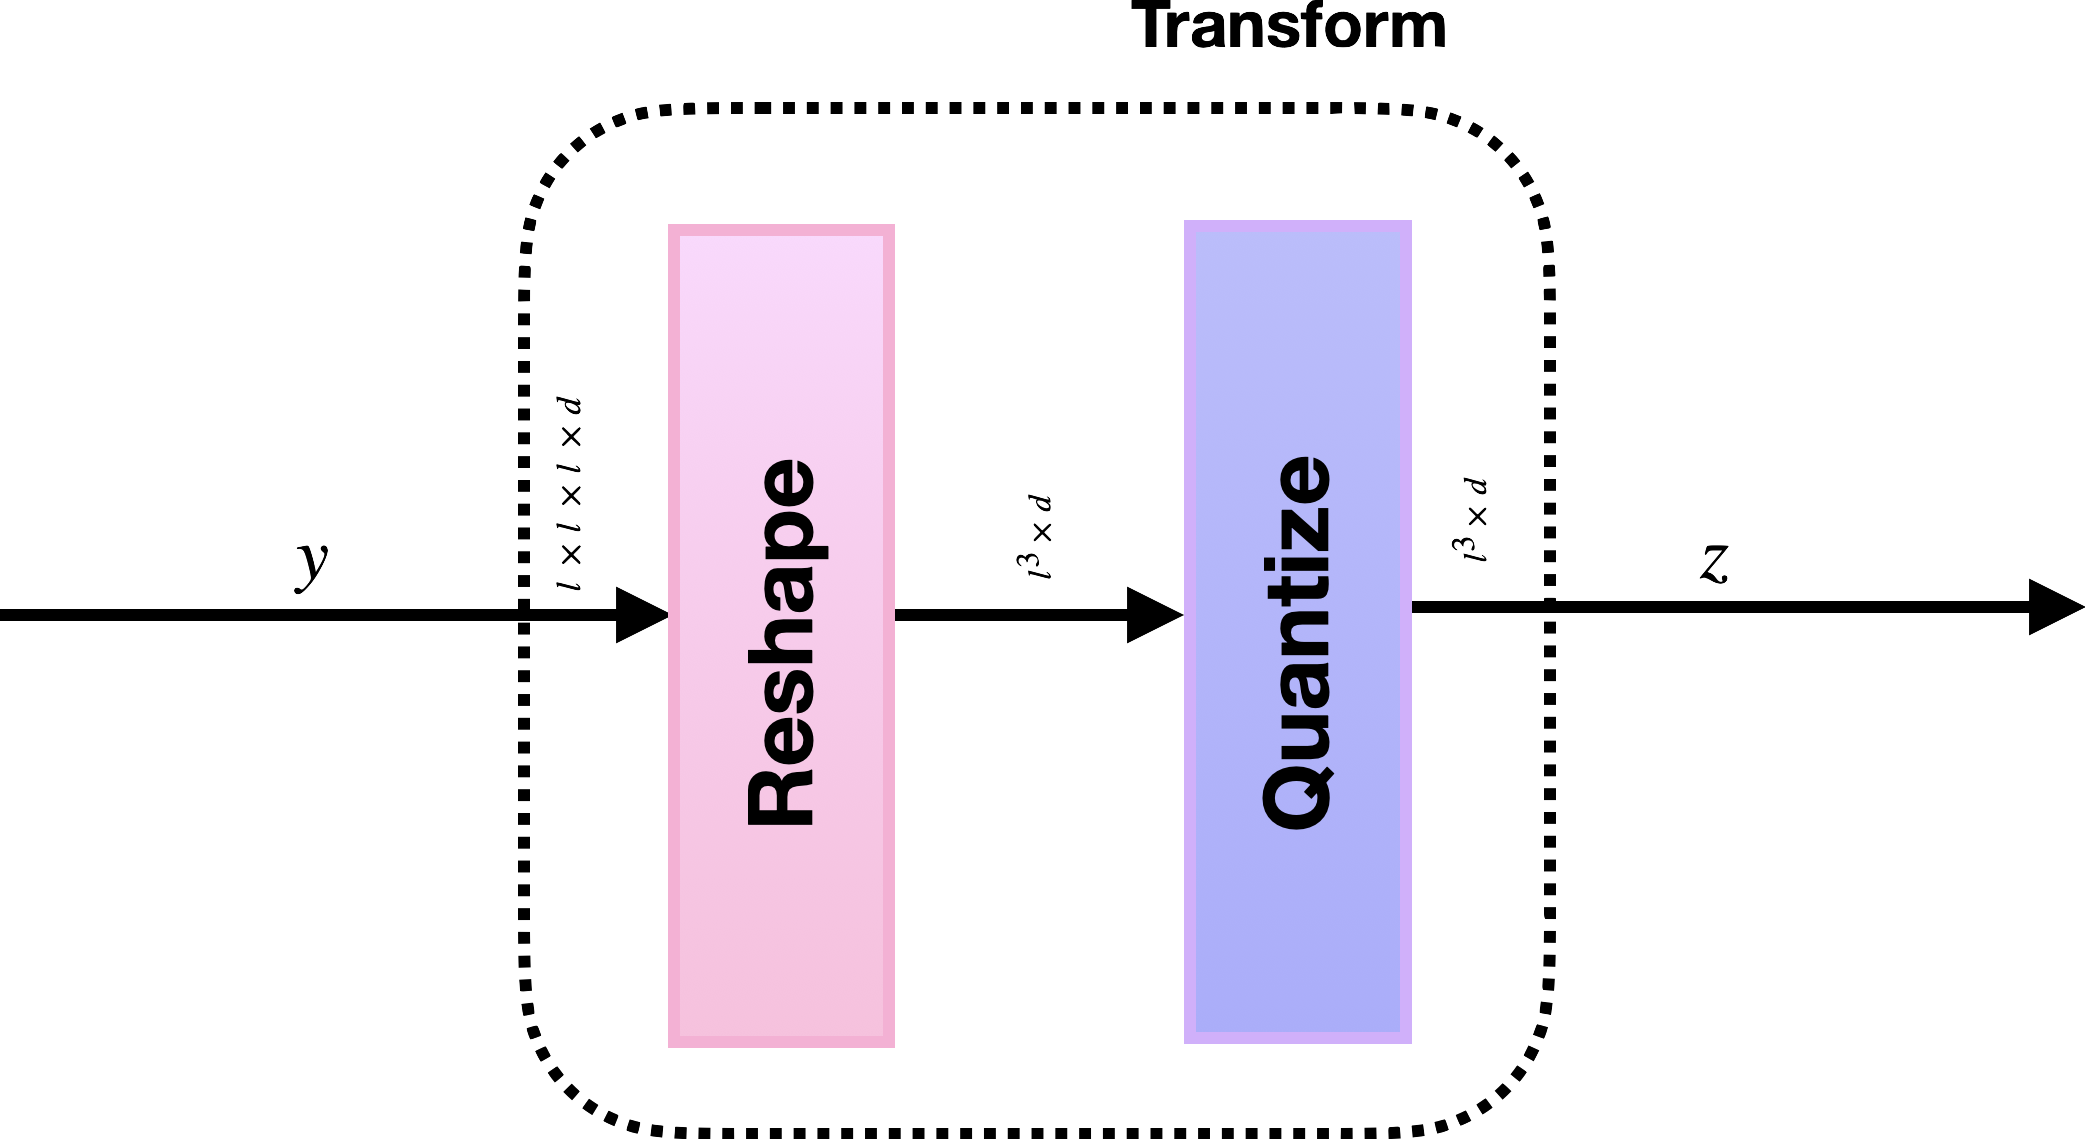
\includegraphics[width=0.5\textwidth]{jpegdna/transform}
    \caption{Reshape + quantization layers}
    \label{fig:reshape+quantization}
\end{figure}

% However, in our case, not dividing by a quantization table is a plus since they are built in order to keep a perceptual fidelity which means that all the high frequency DC are usually dropped and it would affect badly our recovered coefficients and in the end the recovered point clouds because the model is more sensitive to high frequency details than our human eyes.
% 
% In the end, we have a codec that can encode our coefficients in a lossless manner. Unfortunately, one downside of this non DCT codec is that all non-zero coefficients are always encoded and thus never dropped, so we can not control the nucleotide stream length with this method. We will always have the best quality.

\section{Nucleotide stream}

We now have a full pipeline that can be used to encode and decode point clouds. The last step is to produce the actual nucleotide stream from the output of the codec and all intermiediate information that are needed in order to fully decode the stream.

The intermediate informations needed to produce the nucleotide stream are:
\begin{itemize}
    \item The threshold used to turn the reconstructed block $\tilde{x}$ (the probability occupancy grid described in \ref{subsec:model-architecture}) as an \textit{uint8} value;
    \item The oligo length used by the JPEG DNA codec (by default set to 200);
    \item The quantization range used for the latent representation $y$ as described in \ref{subsec:quantization};
    \item The shape of the latent representation $y$ in order to reshape the decoded array of the codec since we merge all inner dimensions together to encode with the codec;
\end{itemize}

To turn a byte array into a nucleotide stream, we naively assume that each two consecutive bits can be considered as a nucleotide. We can use the mapping  
$00 \rightarrow \text{A}$,
$01 \rightarrow \text{C}$,
$10 \rightarrow \text{G}$,
$11 \rightarrow \text{T}$.
With this technique we can produce a $4$ nucleotide stream for each byte of the byte array.

Here is how many nucleotides we can produce to represent our intermerdiate informations:
\begin{itemize}
    \item The threshold is a single byte since it is a \textit{uint8} value $\in [0, 100]$ so we can produce $4$ nucleotides;
    \item The oligo length is also encoded in a single byte, it thus produces $4$ nucleotides as well;
    \item The quantization range are represented as two \textit{float32} values, each value is encoded on $4$ bytes so we can produce a total of $32$ nucleotides for the quantization range;
    \item The shape of the latent representation has the form $l \times l \times l \times d$ and each dimension is encoded on a single byte so we can produce a total of $16$ nucleotides for the shape;
\end{itemize}

The final stream is obtained by concatenating all the additional informations and the nucleotide stream. In the end we have a total of $4 + 4 + 32 + 16 + n$ nucleotides where $n$ is the number of nucleotides produced by the codec.

\section{End-to-end model}

\begin{figure}
    \centering
    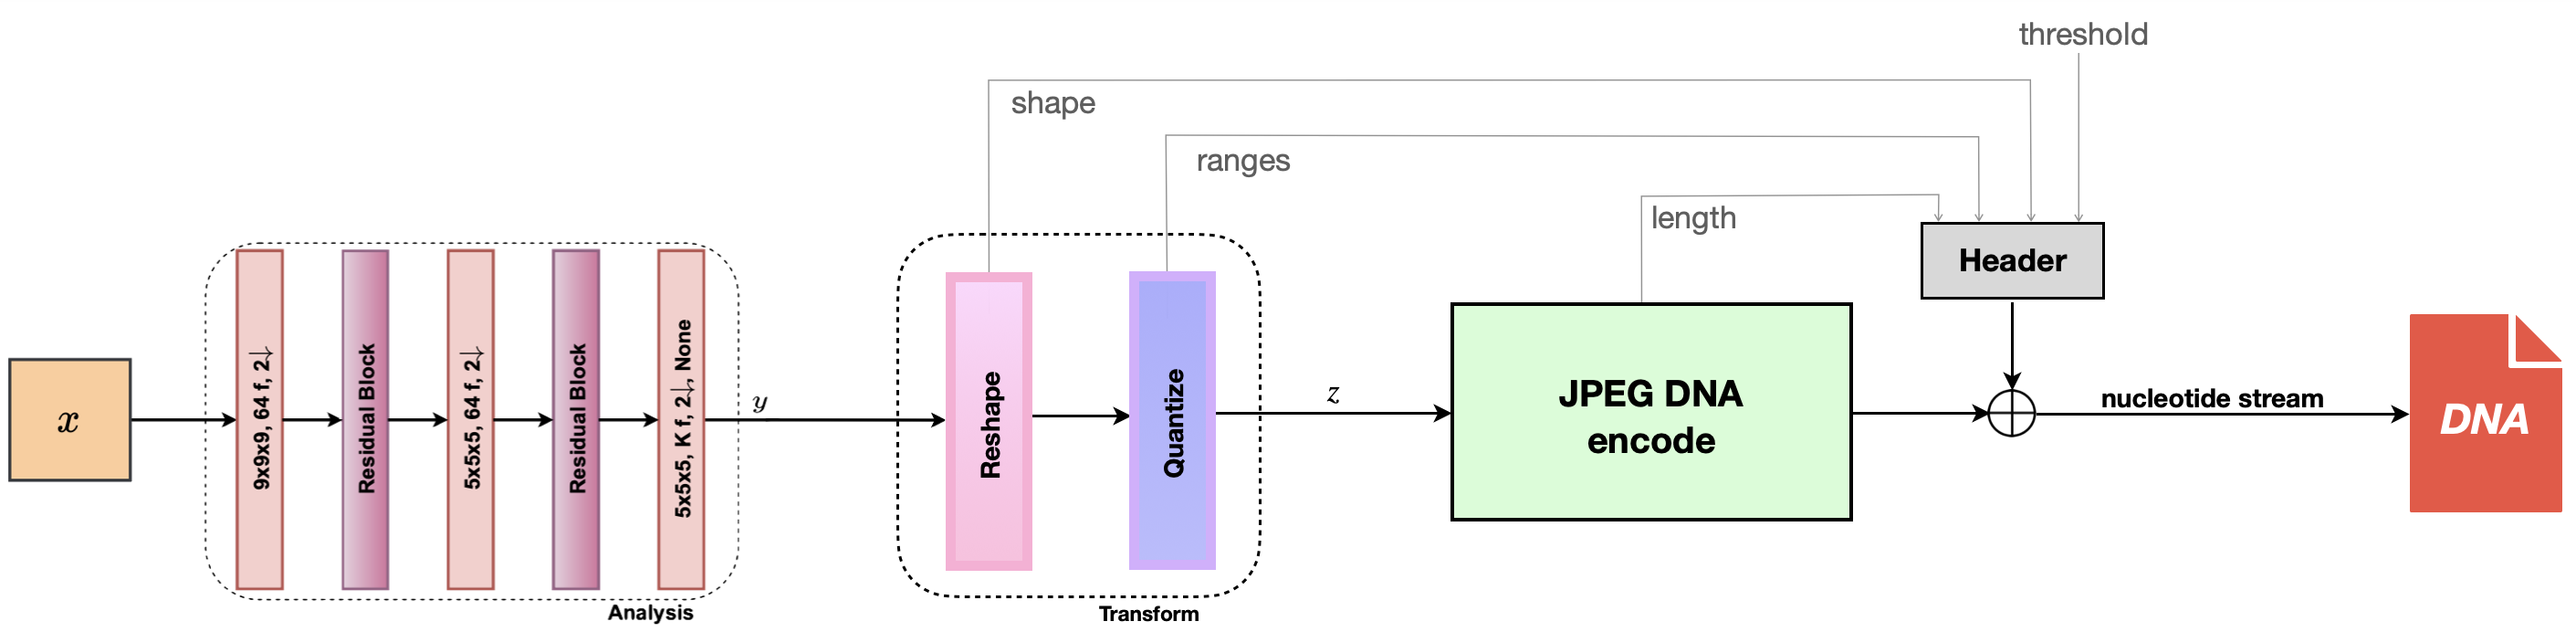
\includegraphics[width=0.95\textwidth]{all}
    \caption{The full end-to-end mode that turns voxelized point clouds into a DNA stream}
    \label{fig:end-to-end}
\end{figure}

With all theses changes, we now have a fully working end-to-end model capable of compressing a voxelized point cloud into a DNA stream respecting some constraints (homopolymers and kmer) thanks to PAIRCODE and the Goldman encoding. The model is shown on Figure~\ref{fig:end-to-end}.

\section{Reconstruction}

Starting from the nucleotide stream, we can fully reconstruct the point doing by doing all steps in reverse order.
First, we extract all the additional informations and the codec stream from the nucleotide stream. Then, we can decode the codec stream to reconstruct the latent representation $\tilde{y}$ and reshape it to the shape that was encoded in the stream.
Then, we can decode the latent representation $\tilde{y}$ using the dequantization transform with the quantization range that was also encoded in the stream in order to obtained the reconstrcuted block $\tilde{x}$
Finally, we can round the probabibility occupancy grid $\tilde{x}$ thanks to the threshold that was encoded in the stream and we can obtain the reconstructed binary occupancy grid.
